\section{Timed Petri Nets}
\label{sec:timed_petri_nets}
	In this nets, each timed transition has an associated a parameter $\tau$ which represents
	the duration of the transition. In order to standardize the mathematical definition we will call 
	\emph{immediate} to those transitions where $\tau$ is zero.
	
	\subsection{Mathematical Definition}
		A \emph{Marked Timed Petri Net} \cite{garciaizquierdo}, is mathematically defined as a 8-tuple as follows:
		\begin{equation*}
			PN = \{P, T, I^-, I^+, H, C, m_0, \Gamma\}
		\end{equation*}
		Where the terms $\{P, T, I^-, I^+, H, C, m_0\}$ represent a marked Petri Net with inhibitors 
		arms and bounded places. $\Gamma$ is a vector composed of the values of duration $\tau$
		associated to each transition.
		
		The meaning of each term of the tuple is:		  
		\begin{itemize}
			\item \textbf{P} is a non-empty finite set of places.
			\item \textbf{T} is a non-empty finite set of transitions.
			\item \textbf{$I^+$} and \textbf{$I^-$} are the possitive and negative incidence matrices.
				\begin{equation*}
					P�T\rightarrow \mathbb{Z}
				\end{equation*}
			\item \textbf{H} is the inhibitors arcs matrix.
				$P�T\rightarrow\{0,1\}$
			\item $m_0$ is the net initial marking.
				$P\rightarrow \mathbb{N}$
			\item $C$ is a vector containing the values that represent the maximum amount of tokens
				that each place of the net can hold.
				$C\rightarrow \mathbb{N}$	
			\item \textbf{$\Gamma$} is the set of static intervals associated with each transition. 
				$T\rightarrow \mathbb{Q}^+ � (\mathbb{Q}^+ \cup \infty)$	
				For each transition \emph{t} the associated value $timer_t$ is:
				\begin{equation*}
					\Gamma (t) = (tau_t \text{ where } t \in T \text{ and } \tau \rightarrow \mathbb{Q}^+
				\end{equation*}
		\end{itemize}
		
		$timer_t$ represents the time elapsed since the firing of the transition start and its value 
		its value is zero at any other moment. $\tau_t$ is the duration of the transition. For that
		reasons, the following conditions must be met:
		\begin{equation*}
			\begin{matrix}
				0 \leq timer_t \leq \tau_t
				\\
				0 \leq \tau_t \leq \infty
			\end{matrix}
		\end{equation*}
		
	\subsection{States of a Timed Petri Net}
		
		In these Petri Nets, the net state is defined by the marking vector ($m=i$) and an 
		\emph{timer} vector that indicates the time stamp of each trasition. Therefore the net 
		state is:
		\begin{equation*}
			S = (m_i,\tau)
			\label{eq:timed_net_state}
		\end{equation*}
			
	\subsection{Sensitization of the Transitions and Firing Rules}
	\label{subsec:sensitization_transitions}
%TODO translate this		
		When we refer to transitions we need to establish the diference between an  enabled or sensitized 
		transition, a not enabled or sensitized transition  and the firing of a transition.

		In a Marked Petri Net whose current mark is $m_k$  we say that a transition $t_j$ is enabled or
		sensitized if and only if $timer_{tj}=0$ and the amount of tokens in all places $p_i$ belonging to
		the set $\bullet t_j$ is at least equal to the weight of the arc that connects them with the
		transition $t_j$ ($w(p_i , t_j)$). Mathematically:
		\begin{equation*}
			\forall p_i \in \bullet t_j : m(p_i) \geq w(p_i,t_j ) \land timer_{tj}=0
			\label{eq:sensitization_conditions}
		\end{equation*}
		
		In summary, every place connected to the transition $t_j$ have at least the number of tokens 
		indicated by the weight of the arc and there is no firing in progress for that transition.
		
		Sensitized transitions can be fired and every time the firing of a transition is completed it
		generates a new marking for the Petri Net. This means that the net changes its state.

		To determine the new state or mark of the net after firing a transition $t_j$, you should the
		\emph{state equation} $\delta(m_k , t_j)$.
		
		\begin{equation*}	
			\delta (m_k,t_j)
				\begin{cases} 
					m_{k+1} (p_i)=m_k (p_i )-W_{ij} & \forall p_i \in \bullet t_j 
					\\ 
					m_{k+1} (p_i)=m_k (p_i )+W_{ij} & \forall p_i \in t_j \bullet \land timer_{tj}=\tau_tj
					\\
					m_{k+1} (p_i)=m_k (p_i ) & \mbox{in the rest of the cases}
				\end{cases}
			\label{eq:state_equations}
		\end{equation*}

		$timer_{tj}$ is incremented in every clock cycle after the firing of the transition started.

	\subsection{Interpretation of the firing of transitions in the system}
		The figure \ref{fig:reactive_systems} represents a reactive systems that responds to events which
		come from the environment, it interacs with the environment. Those events are directed to the Time
		Petri Nets processor.
	
		The responsibility of the processor is arrange events  according to system constraints. These
		constraints are modeled by the TImed Petri Net which is used to program the processor. On the
		other hand, multicore system threads also generate events (to request resources, to synchronize) 
		that are directed to the processor.		
		\begin{figure}[h]
			\centering
			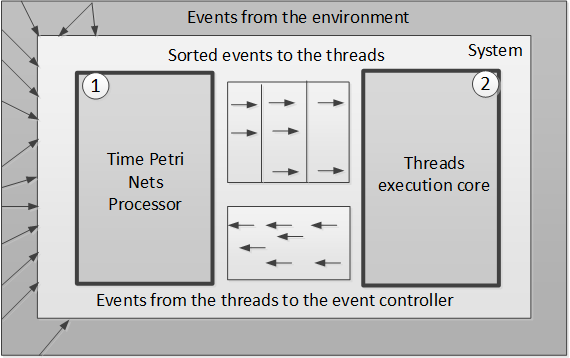
\includegraphics[width=1\linewidth]{reactive_system}
			\caption{Reactive systems}
			\label{fig:reactive_systems}
		\end{figure}
		
		Module 1 from the Figure \ref{fig:reactive_systems} receive unsorted events from the environment
		and from the system itself. After the sorting of the events the Timed Petri Nets processor
		transmits the result to the threads execution cores (module 2) of the system and the propers
		actions are taken. 
			
%TODO No se entiende el significado
\textbf{
No se entiende el significado
\\
Si en nuestro  sistema se asocian el cumplimiento de las condiciones del programa a las que las transiciones 
est�n sensibilizadas, la resoluci�n de un disparo  representaran el cumplimiento de dichas restricciones y si 
asociamos la solicitud de verificaci�n de las condiciones a la solicitud de un disparo, la resoluci�n de un 
disparo comunica que las condiciones se han cumplido.
}		
		
		The conditions to be met for the firing of a transition from Timed Petri Processor are:
		\begin{enumerate}
			\item The transition must comply with sensitization conditions named in Section
				\ref{subsec:sensitization_transitions}.
			\item The shot must be explicitly communicated to the processes or implicitly recorded in the
				module of systolic firings.
			\item Since it is possible that multiple transitions simultaneously satisfy the conditions
				described in paragraphs 1 and 2, the Timed Petri Nets processor will execute first the
				firing with higher priority.
		\end{enumerate}	

		Figure \ref{fig:conection_multicore_system} show us how the Timed Petri Nets processor is conected
		in a multicore system.
	
		In case that the firing of the transition can not be resolve, it is queued in the input queue, as
		shown in Figure \ref{fig:conection_multicore_system}, until the conditions of the system allow
		its resolution. The solution of the firing is notified to threads through the system bus, using
		the output queue. The threads of the system will execute the proper actions as indicated by the
		firings that have been resolved, since the resoluction of the firings depends on the Time Petri
		Nets processor state, which itself represents the state of the system.
	
		\begin{figure}[h]
			\centering
			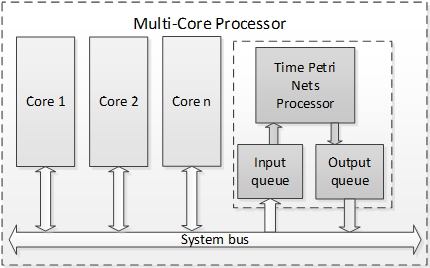
\includegraphics[width=1\linewidth]{conection_multicore_system}
			\caption{Multicore system with Timed Petri Nets processor}
			\label{fig:conection_multicore_system}
		\end{figure}		
		